%        File: hw2.tex
%     Created: Sun Oct 2 05:00 PM 2013 E
% Last Change: Sun Oct 2 05:00 PM 2013 E
%
\documentclass[a4paper]{report}

\title{HW 3}
\author{Delos Chang}
\date{}

\usepackage{amsmath, amsthm, amssymb, fancyhdr, tikz, algorithmicx, algpseudocode, algorithm}
\usetikzlibrary{arrows}
\newcommand{\justif}[2]{&{#1}&\text{#2}}
\renewcommand{\algorithmicforall}{\textbf{for each}}

\pagestyle{fancy}
\rhead{HW 3:  Delos Chang (help from Prof.)}
\begin{document}
  \begin{enumerate}
    %&=& &=& &=& &=& &=& &=& &=& &=& &=& &=& &=& &=& &=& &=& &=& =
    % Question 1 
    %&=& &=& &=& &=& &=& &=& &=& &=& &=& &=& &=& &=& &=& &=& &=& =
    \item
      In a tree, for any two nodes $a$ and $b$, a unique simple path exists from $a$ to $b$. Therefore, let all references to paths
      mean unique simple paths. 

      - Run BFS from any arbitrary node $s$ in the tree $T=(V,E)$. Mark the last-discovered node $u$ in the BFS, 
      $u$ must be a leaf node. 

      - Run BFS starting from node $u$. Mark the last-discovered node as $v$.
      $\delta(u, v)$ is the diameter of the tree $T$. 

      - In the pseudocode, start $main$ with parameters graph $G$ and an arbitrary source vertex.

      \begin{algorithmic}[1]
      \Function{main}{$G(V,E), s: source vertex$}
      \State $u$ = BFS($G$, $s$)
      \State $v$ = BFS($G$, $u$)

      \Comment Return the diameter
      \State return $\delta(u,v)$
    \EndFunction

    \end{algorithmic}
      \begin{algorithmic}[1]
      \Function{BFS}{$G(V,E), s:source vertex$}
      \ForAll{$v \in V$}
        \State d[$v$] = $\infty$
      \EndFor
      \State $d[s] = 0$

      \State Initialize queue Q to contain element $s$
      \While{$Q$ is not empty}
        \State $u = dequeue(Q)$
        \ForAll{$v \in Adj[u]$}
          \If {$d[v] == \infty$}
            \State $d[v] = 1 + d[u]$
            \State enqueue($Q,v)$
          \EndIf
        \EndFor
      \EndWhile
      \Comment $u$ will be the last discovered node
      \State return $u$

    \EndFunction
    \end{algorithmic}

      {\bf Time Complexity }
      BFS has a time complexity of $\Theta(V+E)$. Since it is run twice, the time complexity of this algorithm is still $\Theta(V+E)$ because 
      marking the nodes $u$ and $v$ take $\Theta(1)$ time.


      {\bf Correctness}
      Let $\delta(u,v)$ denote the shortest-path distance between vertex $u$ and vertex $v$.

      Let $(x,y) \in V$ be such that $\delta(x,y)$ is the diameter of tree $G$.

      Let $u$ be the furthest vertex from the source vertex of the first BFS. Then, 

      {\bf Claim}: $\delta(u,x) \geq \delta(x,y)$ or $\delta(u,y) \geq \delta(x,y)$

      
      Let $w$ be the first node on the path from $x$ to $y$ discovered by the first BFS.
      Because $w$ is on the path from $x$ to $y$, $w$ will be a common ancestor to either $x$ and $s$ and/or $y$ and $s$.

      %If the paths $p_{1}$ and $p_{2}$ do share edges, then $t$ is on $p_{1}$. 
      
      Case 1: $w$ is a common ancestor to $x$. 

      Because $u$ is the last and farthest node discovered by the first BFS run on $s$ and $w$ is a node first discovered by BFS,
      no other node can be further from $w$ than $u$ (some node can be of equal distance from $w$ though). Thus: $\delta(w,u) \geq \delta(w,y)$. 

      Because it is given that $\delta(x,y)$ is the longest path and $w$ is an ancestor of $x$, $\delta(w,y) \geq \delta(w, u)$.
      
      Thus, given these two inequalities, $\delta(w, y) = \delta(w, u)$. Therefore, because $w$ is a constant distance from $x$, 
      $\delta(u,x) = \delta(x,y)$. Hence, we have the claim.

      Finally, given the claim, because in BFS, $v$ is the furthest node from $u$, $\delta(u,v) \geq \delta(u,x) = \delta(x,y)$. 
      However, as $\delta(x,y)$ is the diameter, $\delta(x,y) \geq \delta(u,v)$. Therefore, $\delta(u,v) = \delta(x,y)$.  
      Therefore, $(u,v)$ is the diameter of the tree $T$.


      Case 2: $w$ is a common ancestor to $y$.

      Symmetric with Case 1 (except replace all $x$ with $y$ and all $y$ with $x$), the same reasoning applies.



    %&=& &=& &=& &=& &=& &=& &=& &=& &=& &=& &=& &=& &=& &=& &=& =
    % Question 2 
    %&=& &=& &=& &=& &=& &=& &=& &=& &=& &=& &=& &=& &=& &=& &=& =
    \par
    \bigskip

    \item
      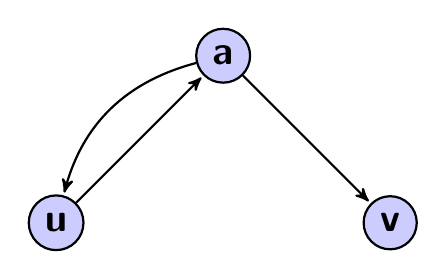
\begin{tikzpicture}[->,>=stealth',shorten >=1pt,auto,node distance=3cm,
        thick,main node/.style={circle,fill=blue!20,draw,font=\sffamily\Large\bfseries}]

        \node[main node] (1) {a};
        \node[main node] (2) [below left of=1] {u};
        \node[main node] (4) [below right of=1] {v};

        \path[every node/.style={font=\sffamily\small}]
        (1) edge node [left] {} (4)
        edge [bend right] node[left] {} (2)
        (2) edge node [right] {} (1);
      \end{tikzpicture}

      Consider a DFS run on the above counterexample directed graph $G$ starting from $a$.  
      There is clearly a path from $u$ to $v$ through $a$ (u $\rightarrow$ a $\rightarrow$ v).

      \begin{center}
        \begin{tabular}{ l | c | r }
          \hline
            & $d$ & $f$ \\ \hline
          $a$ & 1 & 6 \\
          $v$ & 4 & 5 \\
          $u$ & 2 & 3 \\
          \hline  
        \end{tabular}
      \end{center}

      The table shows that $d[u]=2$ and $d[v]=4$, thus $d[u] < d[v]$.

      $v$, however, is not a descendant of $u$ in the depth-first forest produced because the tree edges 
      in the depth-first forest are: $(a,u)$ and $(a,v)$. 

      Hence, the conjecture is disproved with this counterexample.

    %&=& &=& &=& &=& &=& &=& &=& &=& &=& &=& &=& &=& &=& &=& &=& =
    % Question 3 
    %&=& &=& &=& &=& &=& &=& &=& &=& &=& &=& &=& &=& &=& &=& &=& =
    \par
    \bigskip

    \item
      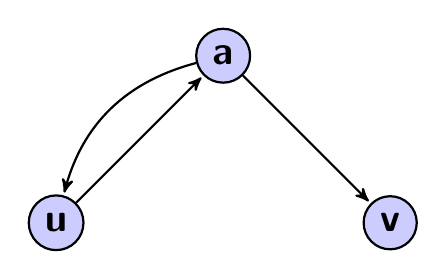
\begin{tikzpicture}[->,>=stealth',shorten >=1pt,auto,node distance=3cm,
        thick,main node/.style={circle,fill=blue!20,draw,font=\sffamily\Large\bfseries}]

        \node[main node] (1) {a};
        \node[main node] (2) [below left of=1] {u};
        \node[main node] (4) [below right of=1] {v};

        \path[every node/.style={font=\sffamily\small}]
        (1) edge node [left] {} (4)
        edge [bend right] node[left] {} (2)
        (2) edge node [right] {} (1);
      \end{tikzpicture}

      Consider a DFS run on the above counterexample directed graph $G$ starting from $a$.  
      There is clearly a path from $u$ to $v$ through $a$ (u $\rightarrow$ a $\rightarrow$ v).

      \begin{center}
        \begin{tabular}{ l | c | r }
          \hline
            & $d$ & $f$ \\ \hline
          $a$ & 1 & 6 \\
          $v$ & 4 & 5 \\
          $u$ & 2 & 3 \\
          \hline  
        \end{tabular}
      \end{center}

      The table shows that $d[v]=4$ and $f[u]=3$, thus $d[v] > f[u]$.

      Hence, the conjecture is disproved because a DFS on $G$ starting from $a$ yields $d[v] > f[u]$.


    %&=& &=& &=& &=& &=& &=& &=& &=& &=& &=& &=& &=& &=& &=& &=& =
    % Question 4 
    %&=& &=& &=& &=& &=& &=& &=& &=& &=& &=& &=& &=& &=& &=& &=& =
    \par
    \bigskip

    \item
      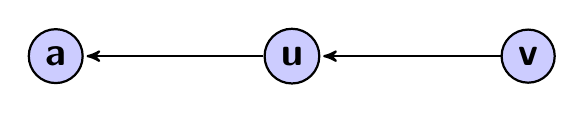
\begin{tikzpicture}[->,>=stealth',shorten >=1pt,auto,node distance=3cm,
        thick,main node/.style={circle,fill=blue!20,draw,font=\sffamily\Large\bfseries}]

        \node[main node] (1) {u};
        \node[main node] (2) [left of=1] {a};
        \node[main node] (4) [right of=1] {v};

        \path[every node/.style={font=\sffamily\small}]
        (4) edge node [left] {} (1)
        (1) edge node [right] {} (2);
      \end{tikzpicture}

      $u$ evidently has both incoming and outgoing edges in $G$ ($u,a$) and ($v,a$).

      Consider a DFS run on the above counterexample directed graph $G$ starting from $a$ with the 
      following discovery and finish times.  

      \begin{center}
        \begin{tabular}{ l | c | r }
          \hline
            & $d$ & $f$ \\ \hline
          $a$ & 1 & 2 \\
          $v$ & 5 & 6 \\
          $u$ & 3 & 4 \\
          \hline  
        \end{tabular}
      \end{center}


      The DFS on $G$ will discover $a$ first then finish $a$. Then discover $u$, then finish $u$ since
      $a$ was discovered already. Finally DFS will discover $v$, then finish $v$.

      Thus, $u$ is neither an ancestor or a descendant of another vertex. The depth-first tree
      will contain only $u$ with no descendants or ancestors. 

      Hence, the conjecture is disproved.

    %&=& &=& &=& &=& &=& &=& &=& &=& &=& &=& &=& &=& &=& &=& &=& =
    % Question 5 
    %&=& &=& &=& &=& &=& &=& &=& &=& &=& &=& &=& &=& &=& &=& &=& =
    \pagebreak
    \par
    \bigskip

    \item
      - We use the parenthesis theorem to check if $u$ is a descendant of $v$. 

      - In a DFS of an undirected graph $G$, every edge of $G$ is either a tree edge or a back edge, which simplifies
      our classification. In the pseudocode, we would remove the $if$ statement checks for a forward edge and cross edge, i.e.
      modify lines (16) and (20) because the control flow would never reach those parts of the if statement in an undirected
      graph $G$.

      \begin{algorithmic}[1]
      \Function{DFS}{$G(V,E)$}
      \ForAll{$u \in V$}
        \State color[$u$] = white
        \State $\pi$[$u$] = nil
      \EndFor
      \State $time=0$


      \ForAll{$u \in V$}
        \If {color[$u$] == white}
          \State DFSVisit($u$)
        \EndIf
      \EndFor

      \Comment Changes made here to list and classify edges
      \ForAll{$(u,v) \in E$}
        \If {$\pi$[$v$] == $u$}
          \State print Tree Edge: ($u$,$v$)
        \Else 
          \Comment Parenthesis theorem to determine ancestry
          \If {d[$u$] $<$ d[$v$] $<$ f[$v$] $<$ f[$u$]}
            \State print Forward Edge: ($u$,$v$)
          \ElsIf {d[$v$] $<$ d[$u$] $<$ f[$u$] $<$ f[$v$]}
            \State print Back Edge: ($u$,$v$)
          \Else
            \State print Cross Edge: ($u$,$v$)
          \EndIf
        \EndIf
      \EndFor

    \EndFunction
    \end{algorithmic}

    The DFSVisit function remains unchanged:

    \begin{algorithmic}
      \Function{DFSVisit}{$u$}
      \State color[$u$] = gray
      \State $time$++
      \State d[$u$] = time

      \ForAll{$v \in $ Adj[$u$]}
        \If {color[$v$] == white}
          \State $pi$[$v$] = $u$
          \State DFSVisit($v$)
        \EndIf
      \EndFor

      \State color[$u$] = black
      \State $time$++
      \State f[$u$] = time
    \EndFunction
    \end{algorithmic}

    %&=& &=& &=& &=& &=& &=& &=& &=& &=& &=& &=& &=& &=& &=& &=& =
    % Question 6 
    %&=& &=& &=& &=& &=& &=& &=& &=& &=& &=& &=& &=& &=& &=& &=& =
    \par
    \bigskip

    \item
      - Initialize a new integer array $count$ where $count[v]$ holds the number of paths from 
      that vertex $v$ to the target vertex $t$. 

      - Initialize all $count$ fields for every vertex to be 0. 

      - Run DFS from the source vertex $s$. When DFS discovers the target vertex $t$,
      set $count[t]$ to 1. Mark $t$ as finished so as to prevent DFS from running from $t$.

      - Each time DFS finishes a vertex $u$, set $count[u]$ to equal the sum of every adjacent
      vertices' $count$.

      - When DFS completes, print $count[s]$ where $s$ is the source vertex.

      \begin{algorithmic}[1]
      \Function{DFS}{$G(V,E)$, $s$: source vertex, $t$: target vertex}

      \Comment Added input parameters
      \ForAll{$u \in V$}
        \State color[$u$] = white
        \State $\pi$[$u$] = nil
        \State $count[u]$ = 0 
      \Comment each vertex's count starts at 0

      \EndFor
      \State $time=0$


      \ForAll{$u \in V$}
        \If {color[$u$] == white}
          \State DFSVisit($u$, $s$, $t$)
        \EndIf
      \EndFor

      \Comment $count[s]$ equals number of paths from $s$ to $t$
      \State return $count[s]$

    \EndFunction
    \end{algorithmic}

    \begin{algorithmic}[1]
      \Function{DFSVisit}{$u$, $s$, $t$}
      \State color[$u$] = gray
      \State $time$++
      \State d[$u$] = time

      \ForAll{$v \in $ Adj[$u$]}
        \If {color[$v$] == white}
          \State $pi$[$v$] = $u$


          \Comment Check if $t$ was discovered
          \If {v == $t$}
            \Comment Stop processing DFS from $t$ 
            \State $count[v]$ = 1
            \State $color[v]$ = black
          \Else
            \Comment Otherwise, continue
            \State DFSVisit($v$)
          \EndIf
        \EndIf

        \Comment add adjacent vertice counts to $u$
        \State $count[u] += count[v]$
      \EndFor

      \State color[$u$] = black
      \State $time$++
      \State f[$u$] = time
    \EndFunction
    \end{algorithmic}

    {\bf Time Complexity:}

    DFS has a time-complexity of $O(|V| + |E|)$ and because this algorithm does not process DFS beyond target vertex $t$, it 
    may explore less of the graph. 

    The modifications: initialization of $count$, returning the final $count[s]$, $if$ statements, summing are all 
    $\Theta(1)$ operations. Each operation does not affect the outer for loop's $\Theta(|V|)$.

    Thus, this algorithm has a time complexity of $O(|V| + |E|)$.

    {\bf Correctness:}

    We show the correctness of the algorithm by proving the loop invariant, then showing that the correctness of the loop
    invariant implies correctness of the algorithm:

    {\bf Loop Invariant:}

    For every black vertex $v$ in the graph $G$, $count[v]$ will hold the number of simple paths from that vertex $v$ to the target 
    vertex $t$. 

    {\bf Base Case:}
    At the start of the loop, all vertices are white, thus the loop invariant holds true because no vertices are black. 

    {\bf Maintenance:}
    Assume that the loop invariant holds at the start of iteration $I'$. Since the iteration $I'$ took place, it follows 
    from the program that a vertex $v$ is marked black at the start of iteration $I''$. 
    Thus, for any adjacent vertex $u$ (adjacent to $v$), $u$ must also be black. The loop invariant specifies that $count[u]$ equals 
    the number of simple paths from $u$ to target vertex $t$. Hence, $\sum$ $_{u\in adj(v)}$ $count[u]$ simple paths 
    exist from $v$ to $t$. Furthermore, setting $count[v]$ to $\sum$ $_{u\in adj(v)}$ $count[u]$ maintains the loop invariant 
    correctly. 

    Hence, we have the loop invariant. 

    {\bf Termination:}
    When the loop terminates, because DFS starts at source vertex $s$, $s$ must be marked black. Therefore, 
    given the loop invariant, $count[s]$ must hold the number of simple paths from the vertex $s$ (the source) to
    the target vertex $t$, which is what the program returns.

    Hence, the post-condition is satisfied.

    %&=& &=& &=& &=& &=& &=& &=& &=& &=& &=& &=& &=& &=& &=& &=& =
    % Question 7 
    %&=& &=& &=& &=& &=& &=& &=& &=& &=& &=& &=& &=& &=& &=& &=& =
    \par
    \bigskip

    \item
      *
      An undirected graph $G = (V,E)$ does not contain a cycle iff a DFS generates no back edges. Furthermore, an undirected
      graph $G$ has only tree edges and back edges. Therefore, two cases will exist:

        - If undirected graph $G$ has a back edge, then it has a cycle. 

        - If undirected graph $G$ has no back edges, it only has tree edges and therefore, is acyclic.

      *
      Thus, the algorithm will run a modified DFS that checks if an edge $(u,v)$ leads to a gray vertex $v$ and not 
      $u$'s parent (because the graph is undirected) in the depth-first forest. 

    {\bf Pseudocode:}

    The main $DFS(G)$ function is left unchanged.

    \begin{algorithmic}[1]
      \Function{DFSVisit}{$u$}
      \State color[$u$] = gray
      \State $time$++
      \State d[$u$] = time
      \ForAll{$v \in $ Adj[$u$]}
        \If {$v \neq \pi[u]$ and $color[v]$ == gray}
          \State return ``cycle exists''
          \Comment Cycle exists: stop the program
          \State sys.exit()
        \EndIf
        \If {$color[v]$ == white}
          \State $pi$[$v$] = $u$
          \State DFSVisit($v$)
        \EndIf
      \EndFor

      \State color[$u$] = black
      \State $time$++
      \State f[$u$] = time
    \EndFunction
    \end{algorithmic}


    {\bf Time Complexity:}
    Case 1: If the algorithm discovers that the graph is acyclic (no back edges), there are at most $|V| - 1$ edges.
    Together with DFS' time complexity of $\Theta(|V| + |E|)$, this case's time complexity is $\Theta(V)$. 

    Case 2: If the algorithm discovers that the graph is cyclic, it has found a back edge. The algorithm stops before 
    checking at most $|V|$ edges. 
    Together with DFS' time complexity of $\Theta(|V| + |E|)$, this case's time complexity is $O(V)$. 

    Therefore, the algorithm's time complexity is $O(V)$ because $O$ in Case 2 is less strict than $\Theta$ in Case 1. 

    -----

    %&=& &=& &=& &=& &=& &=& &=& &=& &=& &=& &=& &=& &=& &=& &=& =
    % Question 8 
    %&=& &=& &=& &=& &=& &=& &=& &=& &=& &=& &=& &=& &=& &=& &=& =
    \pagebreak
    \par
    \bigskip

    Pseudocode for Topological Sort:

    \item
      \begin{algorithmic}[1]
        \Function{TopSort}{$G=(V,E)$}
        \ForAll{$v \in V$}
          \State $inDegree[v]=0$
        \EndFor

        \ForAll{$u \in V$}
          \ForAll{$v \in Adj[u]$}
            \State $inDegree[v]+=1$
          \EndFor
        \EndFor

        \State Initialize queue Q
        \ForAll{$v \in V$}
          \If {inDegree[v] == 0}
            \State enqueue($Q,v$)
          \EndIf
        \EndFor


        \While{$Q$ is not empty}
          \State $u =$ dequeue(Q)
          \State print $u$

          \ForAll{$v \in Adj[u]$}
            \State $inDegree[v] -= 1$
            \If {inDegree[v] == 0}
              \State enqueue($Q,v$)
            \EndIf
          \EndFor
        \EndWhile

        \ForAll{$u \in V$}
        \If {$inDegree[u] \neq 0$}
            \State print ``cycle exists''
          \EndIf
        \EndFor
      \EndFunction
      \end{algorithmic}

      {\bf Time Complexity}
      - In the for loop at (2), we initialize the in-degree of each vertex to 0, taking $\Theta(V)$ time. 

      - In the for loop at (5), we calculate vertices' in-degrees by scanning the adjacency lists of all the vertices and
      adding 1 to the in-degree of each vertex an edge enters. The time complexity is $\Theta(V+E)$ because we visit
      $|V|$ vertices and $|E|$ edges.

      - Initializing the queue at (10) takes $\Theta(1)$

      - We only consider vertices with an in-degree of 0 and enqueueing takes $\Theta(1)$ time. Therefore, this for loop takes
      $\Theta(V)$.

      - In (16), we continuously process vertices of an in-degree of 0. We ``remove'' it by decrementing all adjacent vertices'
      in-degree count by 1. Then enqueue any vertices with in-degree 0 to continue the topological sort. Each enqueue takes
      $\Theta(1)$ time. 

      - The entire while loop takes $\Theta(V+E)$ 
      
        - Each vertex is enqueued and dequeued at most once because it is ``removed'' after decrementing adjacent vertice degrees.
      Vertices are only enqueued if their original in-degree is 0 or if after decrementing, its in-degree goes to 0. Thus, 
      it takes $O(V)$ time to process each vertex.

        - Similarly, because the adjacency list for each vertex is checked at most once, the algorithm takes $O(E)$ time checking
        the adjacency list for adjacent vertices. In total, $O(E)$ time complexity. 

      - The for loop at line (26) takes $\Theta(V)$ time because it must check every vertex for a cycle.

      Hence, the time complexity of this algorithm is $O(V+E)$.

      {\bf Correctness}

      The algorithm correctly topologically sorts graph $G=(V,E)$. 
      
      The correctness follows from the following observations:
      
      Due to the loop at line (5), for all arbitrary edges $(u,v)$ where $u$ enters $v$, $v$ will have an in-degree of at least 1. 
      Furthermore, $v$ will not be outputted until its in-degree is decremented to 0 in line (20). $v$'s in-degree
      will be 0 only if every edge $(u,v)$ entering $v$ is processed before $v$. Hence, the processing of $u$ will 
      output $u$ and remove it. 

      Thus for all arbitrary edges $(u,v)$, the algorithm will output $u$ before $v$, which when looped over all edges in $G$ will
      yield a topological sort. 

      {\bf Cycles}

      If graph $G$ is cyclic, no vertices in cycles are output because cycle in-degrees never decrement to 0. 
      
      Proof by contradiction: Assume that vertices in cycles are outputted. 

      Given the assumption, there must be a first vertex, $u$, in a cycle in $G$ to be outputted. 
      When $u$ is output, $u$'s in-degree must be 0. 
      Because $u$ is in a cycle, at the start of the algorithm, $u$'s in-degree must have been at least 1. Thus, for
      $u$'s in-degree to be 0, it must have been decremented. Suppose $v$ is $u$'s preceding vertex in the cycle. 
      For $u$'s in-degree to be decremented, $v$ must have been processed and outputted before $u$. 
      This contradicts our original assumption that $u$ is the first vertex in the cycle to be outputted. 

      Hence, no vertices in cycles are outputted.

      Otherwise, if graph $G$ is acyclic, all vertices are outputted. 

      




    %&=& &=& &=& &=& &=& &=& &=& &=& &=& &=& &=& &=& &=& &=& &=& =
    % Question 9 
    %&=& &=& &=& &=& &=& &=& &=& &=& &=& &=& &=& &=& &=& &=& &=& =
    \par
    \bigskip

    \item
      No, Prof. Bacon is wrong though he has a great name. Consider the following counterexample:

      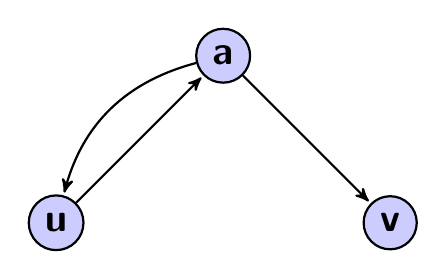
\begin{tikzpicture}[->,>=stealth',shorten >=1pt,auto,node distance=3cm,
        thick,main node/.style={circle,fill=blue!20,draw,font=\sffamily\Large\bfseries}]

        \node[main node] (1) {a};
        \node[main node] (2) [below left of=1] {u};
        \node[main node] (4) [below right of=1] {v};

        \path[every node/.style={font=\sffamily\small}]
        (1) edge node [left] {} (4)
        edge [bend right] node[left] {} (2)
        (2) edge node [right] {} (1);
      \end{tikzpicture}

      By the definition of strongly connected component, because $a$ and $u$ are mutually reachable,
      $\{a,u\}$ are strongly connected components. $\{v\}$ is a strongly connected component because $v$
      is mutually reachable to itself. 

      Assuming $u$ comes before $v$ in $adj[a]$, the following table lists the discovery and finish times:

      \begin{center}
        \begin{tabular}{ l | c | r }
          \hline
            & $d$ & $f$ \\ \hline
          $a$ & 1 & 6 \\
          $v$ & 4 & 5 \\
          $u$ & 2 & 3 \\
          \hline  
        \end{tabular}
      \end{center}

      Thus, the vertices listed in order of $increasing$ finish times is: $\{u, v, a\}$.

      However, calling a second depth-first search scanning vertices in the order $\{u, v, a\}$ colors
      all vertices black in a single loop despite the fact that $\{u, v, a\}$ is not a SCC. 
      In other words, DFS never starts from vertex $v$ because all vertices are colored black after DFS starts from the $u$ vertex. 
      Thus, Professor Bacon's claim would wrongly classify $\{u, v, a\}$ a SCC.

      Hence, the conjecture is disproved with this counterexample.

    %&=& &=& &=& &=& &=& &=& &=& &=& &=& &=& &=& &=& &=& &=& &=& =
    % Question 10 
    %&=& &=& &=& &=& &=& &=& &=& &=& &=& &=& &=& &=& &=& &=& &=& =
    \par
    \bigskip

    \item
        Assume $f(n) = n^k$ for some constant $k$ and $f(n) = \Omega(n^{\log_b a + \epsilon})$ for some constant $\epsilon > 0$.

        For $f(n)$ to hold in both cases, then it must be the case that $k > \log _{b} a$. Otherwise, if $k < \log _{b} a$ and
        $f(n) = n^k$, then by definition, $f(n) \neq \Omega(n^{\log_b a + \epsilon})$.

        $$ k > log_b a$$
        $$ b^k > b^{log_b a} $$
        $$ b^k > a $$
        $$ 1 > \frac{a}{b^k} $$

        Let $c = \frac{a}{b^k}$ because $k, a, b$ are constants.  Thus, plugging in,

        $$ c < 1 $$

        Finally, plugging in $c$ to $c \cdot f(n)$:

        $c \cdot f(n) = \frac{a}{b^k} \cdot n^k$

        $             = a \cdot (\frac{n}{b})^k$

        $             = a \cdot f(\frac{n}{b})$
        because of the given $f(n) = n^k$.

        Hence, the regularity condition holds. 

    %&=& &=& &=& &=& &=& &=& &=& &=& &=& &=& &=& &=& &=& &=& &=& =
    % Question 11 
    %&=& &=& &=& &=& &=& &=& &=& &=& &=& &=& &=& &=& &=& &=& &=& =
    \pagebreak
    \par
    \bigskip

    \item
      % a)

      a) 
      $T(n)$ is in the form of $T(n) = a \cdot T(\frac{n}{b}) + f(n)$.

      $a = 16, b = 4, f(n) = n^2$. $n^{\log_b a} = n^{\log_4 16} = n^2$. 

      Because $f(n) = \Theta(n^{\log_4 16})$, Case (2) (from CLRS) of the Master Method holds. 

      Hence, $T(n) = \Theta(n^2 \log n)$. 


      \bigskip
      % b)

      b) 
      $T(n)$ is in the form of $T(n) = a \cdot T(\frac{n}{b}) + f(n)$.

      $a = 7, b = 3, f(n) = n^2$. $n^{\log_b a} = n^{\log_3 7}$. 

      Thus, $f(n) = \Omega(n^{\log_3 7 + \epsilon})$ when $\epsilon=0.1$ holds because of the fact that
      $\log_3 7 \approx 1.77$. Hence, $f(n) = \Omega(n^{\log_3 7 + \epsilon})$ for some constant $\epsilon>0$ holds.

      From the proof in \#10, because $f(n) = \Omega(n^{\log_3 7 + \epsilon})$ and $f(n) = n^k$ where $k=2$,
      the regularity condition must hold. For example, consider when $c = 7/9$. Note that $c < 1$ which satisfies part of the
      regularity condition. 
      
      Then,
      
      $$7 \cdot f(n/3) = 7/9 \cdot f(n)$$.
      $$\frac{7 n^2}{9}= \frac{7 n^2}{9}$$ 

      Hence, because the regularity condition holds and because $f(n) = \Omega(n^{\log_3 7 + \epsilon})$ for some constant $\epsilon>0$ holds,
      Case 3 (from CLRS) of the Master Method applies and $T(n) = \Theta(f(n)) = \Theta(n^2)$.

      % c)

      \bigskip
      c) 
      $T(n)$ is in the form of $T(n) = a \cdot T(\frac{n}{b}) + f(n)$.
      
      $a = 2, b = 4, f(n) = \sqrt{n}$. $n^{\log_b a} = n^{\log_4 2} = \sqrt{n}$. 

      Because $f(n) = \Theta(n^{\log_4 16})$, $f(n) = \Theta(\sqrt{n})$, Case (2) (from CLRS) of the Master Method holds. 

      Hence, $T(n) = \Theta(\sqrt{n} \log n)$. 

    %&=& &=& &=& &=& &=& &=& &=& &=& &=& &=& &=& &=& &=& &=& &=& =
    % Question 12 
    %&=& &=& &=& &=& &=& &=& &=& &=& &=& &=& &=& &=& &=& &=& &=& =
    \par
    \bigskip

    \item
      % a)

      a) Because $T(n-2)$, it would take $\frac{n}{2}$ levels for $n$ to become some constant like 1 in the recurrence tree. 
      It follows that there will be $\frac{n}{2}$ terms in the recurrence tree (which would be a vertical line of terms). 

      Because $f(n) = n^2$, each level on the recurrence tree would be $(n)^2, (n-2)^2, (n-4)^2\dots)$ with $\frac{n}{2}$ such terms.
      Note that each level's value is at most $n^2$. 

      Thus, $\frac{n}{2}$ number of levels have at most $n^2$ value at each level. 
      The sum of all the terms on all the levels will be at most:

      $$\frac{n}{2} \cdot n^2 = 0.5 \cdot n^3$$

      Hence, we guess the upper bound is $T(n) = O(n^3)$. 

      Consider the halfway point of the recurrence tree. The value at the halfway point will be $(\frac{n}{2})^2$. There will be
      $\frac{n}{4}$ terms from the top of the recurrence tree to this halfway point. Furthermore, each level from the top of the
      recurrence tree to the halfway point of the recurrence tree holds a value of {\bf at least} $(\frac{n}{2})^2$.

      Therefore, the sum of the first half of the recurrence tree will be at least: $(\frac{n}{2})^2 \cdot \frac{n}{4} = \frac{n^{3}}{16}$.

      Hence, we guess the lower bound is $T(n) = \Omega(n^3)$.

      Given our guesses $T(n) = O(n^3)$ and $T(n) = \Omega(n^3)$, by definition, we guess $T(n) = \Theta(n^3)$.
      However, this is only a guess because we do not account for the cost of all the leaves. 
    

  
      Next, we prove our solution correct by the substitution method:

      Guess: $T(n) = \Theta(n^3)$.

      Claim 1: $T(n) = O(n^3)$ i.e. $T(n) \leq c \cdot n^3$ for some constant $c_{0}>0$.

      Claim 2: $T(n) = \Omega(n^3)$ i.e. $T(n) \geq c \cdot n^3$ for some constant $c_{1}>0$.

      Given: $T(n) = T(n-2) + n^2$

      Inductive Hypothesis: Assume $T(n) \leq cn^3$ at all values less than n (i.e. $n-2$, $n-4$ etc.) for some constant $c>0$.
      \begin{align}
        T(n) &= T(n-2) + n^2  \\
        &\leq c(n-2)^3 + n^2  \text{         (by IH)}\\
        &= c(n^2 - 4n + 4)(n-2) + n^2 \\
        &= c(n^3 - 2n^2 - 4n^2 + 8n + 4n - 8) + n^2 \\
        &= c(n^3 - 6n^2 + 12n - 8) + n^2  \\
        &= cn^3 - 6cn^2 + 12cn - 8c + n^2  \\
        &= cn^3 + n(-6cn + 12c + n) - 8c   
      \end{align}

      Consider when the term $(-6cn + 12c + n)$ is negative. Then
      $cn^3 + n(-6cn + 12c + n) - 8c \leq cn^3$.

      For example, consider when $c=3$ and $n = 3$. Then:
      \begin{align}
        3(3)^3 + 3(-54 + 36 + 3) - 24 &\leq 3(3)^3
      \end{align}

      More generally, the term $(-6cn + 12c +n)$ is negative when 
      $c=3$ and $n \geq 3$.

      Furthermore, the term $(-6cn + 12c +n)$ is negative when  
      any $c>\frac{1}{6}$ and all $n \geq \frac{12c}{6c-1}$. 

      We show the base cases where 
      $cn^3 + n(-6cn + 12c + n) - 8c \leq cn^3$ when $n=1$ and $n=2$.

      Suppose $c=1$ and $n=1$. Then $n(-6cn + 12c + n) - 8c$ is negative and 
      $cn^3 + n(-6cn + 12c + n) - 8c \leq cn^3$ holds. Thus, the base case
      is shown for $c=1$ and $n=1$.

      Suppose $c=1$ and $n=2$. Again, $n(-6cn + 12c + n) - 8c$ is negative and 
      $cn^3 + n(-6cn + 12c + n) - 8c \leq cn^3$ holds. Thus, the base case
      is shown for $c=1$ and $n=2$.

      Thus, we have the induction step.

      Hence we have Claim 1 for all $n \geq 1$.
      

      To prove Claim 2, 
      Inductive Hypothesis: Assume $T(n) \geq cn^3$ at all values less than n (i.e. $n-2$, $n-4$ etc.) for some constant $c>0$.
      \begin{align}
        T(n) &= T(n-2) + n^2  \\
        &\geq c(n-2)^3 + n^2  \text{         (by IH)}\\
        &= c(n^2 - 4n + 4)(n-2) + n^2 \\
        &= c(n^3 - 2n^2 - 4n^2 + 8n + 4n - 8) + n^2 \\
        &= c(n^3 - 6n^2 + 12n - 8) + n^2  \\
        &= cn^3 - 6cn^2 + 12cn - 8c + n^2  \\
        &= cn^3 + n(-6cn + 12c + n) - 8c   
      \end{align}
      If $n(-6cn + 12c + n) - 8c \geq 0$, then $cn^3 + n(-6cn + 12c + n) - 8c \geq cn^3$.

      Consider when $c=\frac{1}{6}$ and all $n\geq\frac{2}{3}$. Then, $n(-6cn + 12c + n) - 8c \geq 0$.
      And thus $T(n) \geq cn^3$ when $c=\frac{1}{6}$ and all $n\geq\frac{2}{3}$.

      Hence, we have the induction step and Claim 2.

      Because $T(n) = O(n^3)$ and $T(n) = \Omega(n^3)$, it follows that $T(n) = \Theta(n^3)$.

      % b)
      \bigskip
      b)
      In the recurrence tree, the top level's value is $n$. The second level's value is $\frac{7}{8}n$.
      The third level's value is $(\frac{7}{8})^2n$ and so on.

      The sum of all such terms is a geometric series in the form of 

      $$n(a + ar + ar^2 + \dots) \text{ where } a=1 \text{ and } r=\frac{7}{8}$$

      and the series ends at some term.

      Thus, because the geometric series ends at some definite term ($\log n$ term), the sum must be less than the same geometric series (where 
      where $a=1$ and $r=\frac{7}{8}$) that is {\bf infinite}.

      Because $r < 1$, the sum of an infinite geometric series is $\frac{a}{1-r} = 8$.

      Thus, the sum of all levels of the recurrence tree must be $\leq 8n$. 

      Furthermore, the sum of all levels must be $\geq n$ because $n$ is the recurrence tree's first level value. 

      Given these upper and lower bounds, our guess is $\Theta(n)$.

      Next, we prove our solution correct by the substitution method:

      Guess: $T(n) = \Theta(n)$.

      Claim 1: $T(n) = O(n)$ i.e. $T(n) \leq c \cdot n$ for some constant $c_{0}>0$.

      Claim 2: $T(n) = \Omega(n)$ i.e. $T(n) \geq c \cdot n$ for some constant $c_{1}>0$.

      Induction hypothesis: $T(n) \leq cn$ for some constant $c>0$ at all values less than $n$ (i.e. $n/2$, $n/4$ etc.)

      \begin{align}
        T(n) &= T(n/2) + T(n/4) + T(n/8) + n \\
        &\leq c(n/2)+ c(n/4) + c(n/8) + n\text{         (by IH)}\\
        &= 7cn / 8 + n \\
        &= n \cdot (1 + 7c/8) \\
        &\leq cn \text{    if $c\geq8$}
      \end{align}

      Thus, we have shown that $T(n) \leq cn$ for a $c>0$.

      Hence, we have the induction step and Claim 1, $T(n) = O(n)$. 

      To prove Claim 2, we start with:

      \begin{align}
        T(n) &= T(n/2) + T(n/4) + T(n/8) + n \\
        &\geq n
      \end{align}

      From (21) to (22), we can drop the terms on the right-side to create the inequality. 

      Thus, we have shown that $T(n) \geq cn$ for $c=1$.

      Hence, we have Claim 2, $T(n) = \Omega(n)$.

      Because $T(n) = O(n)$ and $T(n) = \Omega(n)$, it follows by definition that $\Theta(n)$.



  \end{enumerate}
      Let $T_{s}$ denote a tree rooted in the vertex $s$. Note that between any two vertices in tree $T$, there exists
      a unique simple path between them. As such, all references to paths are unique simple paths.

      For every node $v$ in the tree $T$ with children nodes $u_{0}, u_{1}, u_{2} \dots u_{k}$, 
      the diameter of $T_{v}$ will be the max between the following:

      1.the diameter of one of $v$'s subtrees $T_{u_{0}} \dots T_{u_{k}}$.

      2.the longest path between two leaves from two distinct $v$ subtrees $T_{u_{0}} \dots T_{u_{k}}$, 
      passing through and connected by $v$.

      In Case 2, the longest path can be calculated by adding the heights of the two subtrees together. 

      Hence, using the above two cases, we can recursively calculate the diameter of each tree bottom-up. 

      {\bf Time Complexity}
      O(V)


      {\bf Pseudocode}
      - The following psuedocode will store the height of the tree using a pointer. This reduces the 
      time complexity of the algorithm by computing the height of a subtree in the same recursion.
      
      - $height$ should be called initially with 0.


      \begin{algorithmic}[1]
      \Function{calcDiameter}{tree, *height}
      \Comment Set the height of every subtree to 0
      \ForAll{$u \in V$}
        \State $h[u] = 0$
      \EndFor


      \ForAll{$u \in V$}
        \If {color[$u$] == white}
          \State DFSVisit($u$)
        \EndIf
      \EndFor

      \Comment Changes made here to list and classify edges
      \ForAll{$(u,v) \in E$}
        \If {$\pi$[$v$] == $u$}
          \State print Tree Edge: ($u$,$v$)
        \Else 
          \Comment Parenthesis theorem to determine ancestry
          \If {d[$u$] $<$ d[$v$] $<$ f[$v$] $<$ f[$u$]}
            \State print Forward Edge: ($u$,$v$)
          \ElsIf {d[$v$] $<$ d[$u$] $<$ f[$u$] $<$ f[$v$]}
            \State print Back Edge: ($u$,$v$)
          \Else
            \State print Cross Edge: ($u$,$v$)
          \EndIf
        \EndIf
      \EndFor

    \EndFunction
    \end{algorithmic}
\end{document}


